\documentclass[12pt]{article}
\usepackage{graphicx}

\usepackage{tikz}
\usetikzlibrary{positioning}

\begin{document}

\section{Use calc library for distance calculation}

Include the tikzlibrary calc and use the syntax \$(point)!0.5!(point)\$ e.g. to get half
the distance between two points.
Do not cheat! When the distance changes, it should automatically scale.

\noindent The star is at 40\% between top and bottom, the arrow starts at 60\%.
\vspace{1em}

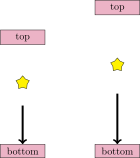
\includegraphics{_img_src/calc.pdf}

\vspace{1em}
\hrule 
\vspace{1em}

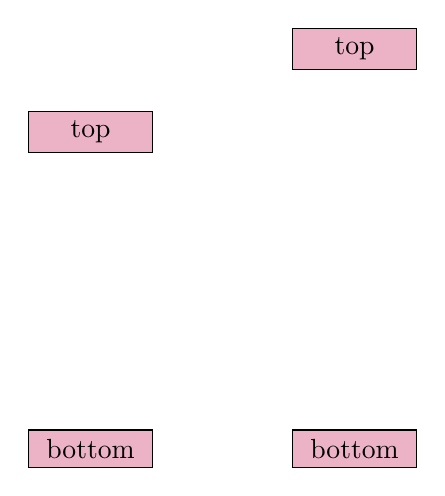
\begin{tikzpicture}

    \node[draw, minimum width=45pt, fill=purple!30] (top) {top};
    \node[draw, minimum width=45pt, fill=purple!30, below=100pt of top] (bottom) {bottom};

    \node[draw, minimum width=45pt, fill=purple!30, right=50pt of bottom] (bottom2) {bottom};
    \node[draw, minimum width=45pt, fill=purple!30, above=130pt of bottom2] (top2) {top};

    %%%%%%%%%%%%%%%%%%%%%
    % Add your code here
    %%%%%%%%%%%%%%%%%%%%%
    
\end{tikzpicture}
\end{document}